\documentclass[12pt]{extarticle}
\usepackage[utf8]{inputenc}
\usepackage[utf8]{inputenc}
\usepackage{tikz}
\usetikzlibrary{er,positioning,bayesnet}
\usepackage{multicol}
\usepackage{xcolor}
\usepackage{algpseudocode,algorithm,algorithmicx}
\usepackage{hyperref}
\usepackage[inline]{enumitem} % Horizontal lists
\usepackage{cite}
\usepackage{amsmath}
\usepackage{amssymb}
\usepackage{graphicx}
\usepackage{multirow}
\usepackage{booktabs}
\usepackage[labelfont=bf,font=scriptsize]{caption}
\usepackage[font=scriptsize]{subcaption}
\usepackage{mhchem}
\newcommand{\indentitem}{\setlength\itemindent{20pt}}
\newcommand{\F}{\ensuremath{\mathbb{F}}}
\newcommand{\B}{\ensuremath{\mathbb{B}}}
\newcommand{\LL}{\ensuremath{\mathbb{L}}}
\renewcommand{\d}{\ensuremath{\text{d}}}
\title{Polyelectrolytes Model Derivation}
\author{}

\begin{document}
\section{Polyelectrolytes Gel Model Derivation.}
\label{modeldev}
\subsection{Conservation Law.}
\label{conslaw}
We here consider the gel as a three-phase medium composed of a solid polymer network with fixed charges, a solvent (i.e. water molecules, interstitial fluid) and solutes (freely moving charges). 
\begin{figure}[h!]
	\centering
	\def\svgwidth{0.9\linewidth}
	\input{images/deformation.pdf_tex}
	\caption{Sketch of the dry and current state of the gel.}
	\label{Above}
\end{figure}

As the tissue deforms, the material element originally located at $\mathbf{X}$ in the initial configuration $\mathcal{B}_0$ is displaced to the point $\mathbf{x}$ in the current configuration $\mathcal{B}_t$, see Figure \ref{Above}. Such a transformation is described by the deformation gradient tensor $\F= \partial \mathbf{x}/\partial \mathbf{X}$; the information about the change in volume is encoded in $J= \det \F$, while $\mathbf{u}= \mathbf{x}-\mathbf{X}$ is the displacement vector. As in \cite{sarah}, we consider the reference, or initial, state $\mathcal{B}_0$, which is stress free, to be equivalent to the dry state of the gel, i.e. only solid phase present. Since we assume the solid phase to be incompressible, any change in the volume can only be related to the migration of solvent and solute molecules, whose nominal \footnote{variable value in the reference configuration.} concentrations will be denoted by $C_s$ and $C_i$ respectively, $i=1,\ldots,N$ with $N$ being the number of free ion species. This lead to the molecular incompressibility condition:

\begin{equation}
 J= 1 + v_s C_s +\sum\limits_{i=1}^{N} v_i C_i
 \label{comp}
\end{equation}
where $v_m$ are the characteristic molecular volume of each species in the solution. When considering the interstitial fluid, the contribution of ions to the volume can be neglected \cite{ecm1,ecm2} so that Equation~(\ref{comp}) reduces to:

\begin{equation}
J=1+v_s C_s.
\label{inc}
\end{equation} 

Consequently, the volume fractions of fluid $\phi_f$ and solid $\phi_n$ phases in the swollen gel are defined as:
\begin{equation}
\phi_f = \frac{v_sC_s}{1+v_sC_s}, \qquad \phi_n = \frac{1}{1+v_sC_s}.
\end{equation}
where again we are neglecting the contribution of ions to the total volume.
While $C_m$ denotes the number of each molecule per unit volume in the initial configuration for the $m$-th species in the solution, the actual concentration in the current state is denoted by $c_m=C_m/J$. Throughout the derivation of the model, we will be using the index $i=1,\ldots,N$ to denote the ionic species only, while $m\in\left\{s,1,\ldots,N\right\}$ refers to all mobile species, i.e. both the solvent and solutes.

Mass conservation must apply to all mobile species and in the initial configuration this reads:
\begin{equation}
\dot{C}_m + \nabla_0 \cdot \mathbf{J}_m = 0, \label{consmass}
\end{equation}
where $\mathbf{J}_m$ is the nominal flux per unit area in the dry state, $\dot{C}_m$ is the derivative of $C_m$ with respect to time, i.e.  $\dot{C}_m\equiv\partial_t C_m$ and $\nabla_0$ denotes the gradient in the Lagrangian coordinates $\mathbf{X}$. Their counterparts in the actual configuration are denoted by $\mathbf{j}_m$ and $\nabla$ and are defined according to the following rules:
\begin{equation}
\mathbf{J}_m = J \F^{-1} \mathbf{j}_m, \qquad \nabla_0 (\cdot) = \F^{T} \nabla(\cdot).
\end{equation}

When considering tissues or hydrogels, inertial and gravitational effects are commonly neglected, so that the conservation of momentum for the gel reads:

\begin{gather}
\nabla_0 \cdot \mathbb{S}=0\label{consmom},
\end{gather}

where $\mathbb{S}$ is the first Piola-Kirchoff tensor, which represents the stress state of the gel in the initial configuration. The counterpart in the current configuration is the Cauchy stress tensor $\mathbb{T}$, which is related to $\mathbb{S}$ as follows:

\begin{equation}
\mathbb{T} = J^{-1}\mathbb{S}\F^T.\label{TS}
\end{equation}

The presence of free moving ions generates an electric field which is denoted by $\mathbf{E}$ and $\mathbf{e}$ in the initial and current configuration respectively. Introducing the electrostatic potential $\Phi$, we have that:
\begin{equation}
\mathbf{E}= -\nabla_0 \, \Phi, \hspace{8mm} \mathbf{e}= - \nabla \, \Phi.
\label{Phi}
\end{equation}

As in \cite{Reviewpolyel}, we consider the gel to be a dielectric material\footnote{a material that does not conduct electricity but can be polarized in the presence of an electric field.}. Consequently, the presence of the electric field generates an electric displacement $\mathbf{H}$\footnote{the vector field that accounts for both the electric field and the polarization of the dielectric material.}, which must obey Gauss law of electrostatics:
\begin{equation}
\nabla_0 \cdot \mathbf{H}= Q,
\label{gauss}
\end{equation}
where $Q$ is the local total charge, which accounts for both fixed and moving charges:
\begin{equation}
Q = e\left(\sum\limits_{i} z_i C_i+z_f C_{f}\right)\, , 
\end{equation}
where $e$ is the elementary charge, $C_f$ is the concentration of fix charges and $z_m$ is the valence of the corresponding charged species. As for above, we can move from nominal quantities to the corresponding value in the current configuration by applying the following rules:

\begin{eqnarray}
\mathbf{H} = J \F^{-1}\mathbf{h},\\
\mathbf{E} = \F^T \mathbf{e},
\end{eqnarray}
where $\mathbf{h}$ is the electric displacement in the current configuration.
\subsection{Energy Balance Inequality.}
\label{sec_ine}
The energy imbalance inequality reads:
\begin{equation}
\frac{\d}{\d t} \left\{\int_R \psi \right\}\leq W(R) + M(R) \label{energyin}
\end{equation}
where $R$ is an arbitrary control volume of the system, $\psi$ is the Helmholtz free energy, $W(R)$ is the rate at which the environment does work on $R$ and $M(R)$ is the inflow of mass due to transport. Considering a control volume $R$ in the reference configuration $\mathcal{B}_0$, the system exchanges mass due to the diffusion of each mobile species, so that $M(R)$ is given by:
\begin{equation}
M(R)= \sum\limits_{m=s,1,\ldots,N} - \int_{\partial R} \mu_m \,\mathbf{J}_m \cdot \mathbf{n} 
\end{equation}
where $\mathbf{n}$ is the unit normal vector to the surface $\partial R$ and $\mu_m$ is the chemical potential associated with each species. Widely used in the thermodynamics of mixture, the chemical potential is a measure of the rate of change in free energy associated with adding one more molecule to a unit volume.

The term $W(R)$, i.e. the rate of work done on the system, is instead decomposed in two contributions, the rate of electrical $W_{el}(R)$ and mechanical work $W_{mec}(R)$. Following \cite{DROZDOVph}, $W_{el}(R)$ is defined as:
\begin{equation}
W_{el}(R) = -\int_{\partial R} \Phi\, \dot{\mathbf{H}}\cdot \mathbf{n}
\end{equation}

Following the work of Gurtin \cite{GURTIN}, we account both for the presence of macro-stresses $\mathbb{S}$ and micro-stresses $\boldsymbol{\xi}$, which arise due to the system heterogeneity \cite{microstress}\footnote{Assuming only interface is between solid and solvent phase.}. As before we only consider the dominant contribution of the solvent while neglecting the solute, so that $W_{mec}(R)$ reads:
\begin{equation}	\centering
%	\begin{subfigure}{0.32\textwidth}
%		\centering
%		\Large
%	\def\svgwidth{0.95\linewidth}
%	\input{latex/images/modelA1.pdf_tex}
%	\caption{Rheological Model A}
%	\label{fig1A}
%	\end{subfigure}
W_{mec}(R) = \int_{\partial R} \left(\boldsymbol{\xi}\cdot \mathbf{n}\right)\dot{C}_s + \int_{\partial R} \mathbb{S}\mathbf{n} \cdot \dot{\mathbf{u}}
\end{equation}
where $\mathbf{u}= \mathbf{x}-\mathbf{X}$ is the displacement vector, which is related to the deformation tensor by $\F=\mathbb{I}-\nabla_0 \mathbf{u}$. Substituting this result back into the formula~(\ref{energyin}) and applying the divergence theorem we obtain the following inequality:
\begin{equation}
\int_R \dot{\psi} - \mathbf{E}\cdot \dot{\mathbf{H}} \, + \, \sum\limits_{i=1}^{N} \left[e \Phi  z_i \dot{C}_i+ \nabla_0 \left(\mu_i \mathbf{J}_i \right)\right] + \nabla_0 (\mu_s \mathbf{J}_s- \boldsymbol{\xi}\dot{C}_s -\mathbb{S}^T\mathbf{\dot{u}}) \leq 0 
\end{equation}

Since this must hold for any choice of the volume $R$, the inequality must hold also locally:
\begin{equation}
\dot{\psi} - \mathbf{E}\cdot \dot{\mathbf{H}} \, + \, \sum\limits_{i=1}^{N} \left[e \Phi  z_i \dot{C}_i+ \nabla_0 \left(\mu_i \mathbf{J}_i \right)\right] + \nabla_0 (\mu_s \mathbf{J}_s- \boldsymbol{\xi}\dot{C}_s -\mathbb{S}^T\mathbf{\dot{u}}) \leq 0. 
\end{equation}
Further accounting for Equations~(\ref{consmass})-(\ref{consmom}), we obtain that:
\begin{equation}
\begin{aligned}
\dot{\psi} - \mathbf{E}\cdot \dot{\mathbf{H}} \, + \, \sum\limits_{i=1}^{N} \left[e \Phi  z_i - \mu_i\right] \dot{C}_i - (\mu_s + \nabla_0 \cdot \boldsymbol{\xi})\,\dot{C}_s -\mathbb{S}:\dot{\F}\\
-\boldsymbol{\xi} \cdot \nabla_0 \, \dot{C}_s + \sum\limits_{m} \nabla_0 \, \mu_m \cdot \mathbf{J}_m \leq 0.
\label{temp2}
\end{aligned} 
\end{equation}

As exhaustively discussed in previous studies \cite{Plasto,GURTIN}, the energy inequality imposes restrictions on the constitutive equation of the free energy $\psi$. Adapting their results to our specific problem, we have that:
\begin{equation}
\psi = \psi (\F,\F_e, C_s, C_i, \nabla_0 \,C_s,\mathbf{H}), \label{temp1}
\end{equation}
which precludes any explicit dependency of $\psi$ on the chemical potential or the viscous deformation gradient $\F_v$. By differentiating the incompressibility condition~(\ref{inc}), we obtain:

\begin{gather}
\sum_m v_m\dot{C_m} - J \F^{-T}:\dot{\F} =0, \label{temp3}
\end{gather}

If we now substitute~(\ref{temp1}) into~(\ref{temp2}), and include the constraint~(\ref{temp3}) using as Lagrange multipliers $p$, we are left with the augmented form of the energy imbalance inequality:
\begin{equation}
\begin{aligned}
\color{blue}{\left(\frac{\partial \psi}{\partial \nabla_0 C_s}-\boldsymbol{\xi}\right)} \color{black}\cdot \nabla_0 \dot{C}_s + \color{blue}{\left(\frac{\partial \psi}{\partial C_s}-\mu_s-\nabla_0 \cdot \boldsymbol{\xi}+p v_s\right)}\color{black}\dot{C}_s\\
+ \sum_i\color{blue}\left(\frac{\partial \psi}{\partial C_i} + e\Phi z_i-\mu_i+pv_i\right) \color{black}\dot{C}_i +\color{blue}\left(\frac{\partial \psi}{\partial \mathbf{H}}-\mathbf{E}\right) \cdot \color{black}\dot{\mathbf{H}}\\
+ \color{blue} \left(\frac{\partial \psi}{\partial \F} - \mathbb{S} - p J \F^{-T}\right): \color{black}\dot{\F}+ \sum_m \nabla_0 \,\mu_m \cdot \mathbf{J}_m \leq 0 . \label{ineq}
\end{aligned}
\end{equation}

\subsection{Construction of the Free Energy.}

Having the general form of $\psi$, Equation~(\ref{temp1}), it remains to construct its precise form. Following a standard approach in $\psi$-depending modeling, we assume that the total free energy can be additively decomposed with each physical mechanisms contributing independently. We here consider six distinct contributions:

\begin{enumerate}
	{\indentitem\item[\textbullet] the energy of the electric field $\psi_1$;}
	{\indentitem \item[\textbullet] the energy of solvent and solutes' molecules not interacting with the solid phase $\psi_2$;}
	{\indentitem\item[\textbullet] the energy of mixing the solid phase with the solution, $\psi_3$;}
	{\indentitem\item[\textbullet] the energy of mixing the solvent with the solutes in solution, $\psi_4$;}
	{\indentitem\item[\textbullet] the interfacial energy between dissimilar phases, $\psi_5$;}
	{\indentitem\item[\textbullet] the energy of the solid phase not interacting with the solution, $\psi_6$.}
\end{enumerate}

Assuming the solid phase to be an ideal and linear dielectric material, with constant permittivity $\epsilon$,the free energy of polarization reads \cite{DROZDOV+,Reviewpolyel}:
\begin{gather}
\psi_1 = \frac{1}{2\epsilon J} \mathbf{H}\F^T \cdot \F \mathbf{H}.
\end{gather}

The specific energy density $\psi_2$ has the standard form:
\begin{equation}
\psi_2 = \sum\limits_{m} \mu^0_m C_m
\end{equation} 
where $\mu^0_m$ denotes the chemical potential of non interacting solvent and ions molecules. According to Flory-Huggins theory \cite{flory,hug} of mixtures, the mixing energy is given by:
\begin{equation}
\psi_3 = \frac{k_B T }{v_s} \left(v_sC_s \ln \frac{v_sC_s}{1+v_sC_s} + \chi \frac{v_sC_s}{1+v_sC_s}\right),\label{mix}
\end{equation}
where $k_B$ is the Boltzmann's constant, $T$ is the temperature and $\chi$ is the Flory-Huggins parameter, which is a measure of the enthalpy of mixing. 

Assuming the solution is dilute, the contribution $\psi_4$ reads \cite{Reviewpolyel,ecm1,ecm2}:
\begin{equation}
\psi_4 = k_B T \sum\limits_{i=1}^{N} C_i \left(\ln \frac{C_i}{ C_s}-1\right).
\end{equation}

For non dilute solution the form proposed by Hong \cite{Reviewpolyel} is:
\begin{equation}
\psi_4 = k_B T \sum\limits_{m} C_m \left(\ln \frac{C_m}{\sum_i C_i+C_s}-1\right).
\end{equation}

As proposed by Hong et al. \cite{Interface}, we include in the energy the effect of interface tension. Assuming that the contribution of mobile ions is negligible, only the solid-solvent interface contributes to the energy:
\begin{equation}
\psi_5 = \frac{\gamma}{2} J \left|\nabla C_s\right|^2,
\end{equation}
where the constant $\gamma$ plays a role analogous to a surface tension.

For the strain energy we consider the gel to be an hyper-elastic Neo-Hookean material:

\begin{equation}
\psi_6(\F) = \frac{G}{2} \left(\F:\F - 3 -2 \ln J\right)\
\end{equation}
where $G$ is the shear constant of the material.

\subsection{Entropy Production $\sigma$.}
\label{ent}

Having specified how the system interacts with its environment, we can now discuss how it dissipates energy. We here consider only the contribution due to the transport of the solution(diffusion of solvent and solutes). The thermodynamic fluxes associated with these two phenomena are $\mathbf{J}_m$, $m=s,1,\ldots,N$, and $\LL_v$. Consequently, the entropy production is of the form:

\begin{equation}
\sigma = \sum_m \zeta_m \cdot \mathbf{J}_m,
\label{dis}
\end{equation}
where $\zeta$s represent the thermodynamic forces associate with each flux. On the other hand, $\nabla_0 \dot{C}_s$, $\dot{C}_s$, $\dot{C}_i$, $\mathbf{\dot{H}}$ and $\dot{\F}$ are the independent physical variables that describe the evolution of reversible process. In order for the energy imbalance inequality~(\ref{ineq}) to hold for any choice of the these fields and given the constraint~(\ref{temp1}) on $\psi$, we have that the terms highlighted in blue in Equation~(\ref{ineq}) must be identically zero. 
\begin{gather}
\boldsymbol{\xi} = \gamma J \,\mathbb{B}^{-1} \,\nabla_0 \,C_s,\label{sys1}\\[2mm]
\begin{aligned}
\mu_s = p v_s + \mu_s^0 - \gamma J \nabla^2 C_s + k_BT\left[\ln \frac{C_s v_s}{1+C_s v_s} + \frac{1}{1+C_sv_s}\right.\\
\left.\ \ \ \ \ \ +\frac{\chi}{(1+C_s v_s)^2} + \ln \frac{v_s C_s}{\sum_m v_mC_m} - \frac{v_s \sum_\alpha C_\alpha}{\sum_m C_m v_m} \right], 
\end{aligned}\label{gov1}\\[2.5mm]
\mu_i = p v_i + \mu^0_i + e\Phi z_i + k_BT \ln \frac{v_iC_i}{\sum_m v_m C_m} - k_BT \frac{\sum_a C_a v_i}{\sum_m v_m C_m},\label{mu}\\
\mathbf{E} = \frac{1}{\epsilon J} \F^T \F\, \mathbf{H}\, , \qquad -\epsilon J \nabla^2 \Phi = Q\, ,\label{sys2}
\end{gather}
\begin{gather}
\begin{aligned}
\mathbb{T}= -p \mathbb{I} + \underbrace{\gamma \left[\frac{1}{2} |\nabla C_s|^2\mathbb{I} - \nabla C_s \otimes \nabla C_s\right]}_{\mathbb{T}^{kort}}+ \underbrace{\epsilon \left[\frac{1}{2} \,|\nabla \Phi|^2\mathbb{I} -\nabla \Phi \otimes \nabla \Phi\right]}_{\mathbb{T}^{Max}}\\
+ \frac{G}{J}\left(\mathbb{B}-\mathbb{I}\right),
\end{aligned}
\label{sys3}
\end{gather}

So that the energy imbalance inequality reduces to:
\begin{equation}
\sum_m \nabla_0 \,\mu_m \cdot \mathbf{J}_m \leq 0.
\end{equation}
In the framework of linear non-equilibrium thermodynamics, when considering isothermal transformation, the second law of thermodynamics can be rewrite as:
\begin{equation}
W(R)+M(R)-\frac{\d}{\d t} \left\{\int_R \psi \right\} = T \int_R \sigma \,\d V\, ,
\label{eqCIT}
\end{equation}

Substituting Equations~(\ref{sys1})-(\ref{sys3}) into~(\ref{eqCIT}) and moving from the integral to the local form, we obtain:
\begin{equation}
\begin{aligned}
\sigma = -  \sum_m \frac{1}{T}\nabla_0 \,\mu_m \cdot \mathbf{J}_m. \label{EQen}
\end{aligned} 
\end{equation}

Comparing Equation~(\ref{EQen}) and~(\ref{dis}), it is evident that the thermodynamics forces are:
\begin{equation}
\zeta_m = -\frac{1}{T} \nabla_0 \,\mu_m. \label{vflow1}
\end{equation}
Assuming to be in regime of linear non-equilibrium thermodynamics, we have that forces linearly depend on fluxes:
\begin{equation}
\zeta_k = -\frac{1}{T} \nabla_0 \,\mu_m =\sum_{k=s,1,\ldots,N} H_{mk} \mathbf{J}_m. \label{dif}
\end{equation}

Since the entropy production depends on the deformation, it is more suitable to move from the Lagrangian to the Eulerian coordinates. So that Equation~(\ref{dif}) can be rewritten as:
\begin{equation}
\nabla \,\mu_m  = - \sum_{k=s,1,\ldots,N} T J H_{mk} \mathbb{B}^{-1} \, \mathbf{j}_m= \sum_{k=s,1,\ldots,N} \ell_{mk}\   \mathbf{j}_m. \label{dif2}
\end{equation}
where the coefficient $\ell_{mk}$ are now constant, i.e. they are independent of the deformation. These can be correlated to drag coefficients, which are commonly used in the theory of mixtures \cite{ecm1,ecm2}. Let us first rewrite the fluxes as $\mathbf{j}_m = c_m (\mathbf{v}_m-\mathbf{v}_n)= c_m \bar{\mathbf{v}}_{m}$, where $\mathbf{v}_m$ is the velocity of the $m$-th component in the current configuration, $\mathbf{v}_n$ is the velocity of the network also in the current configuration and  $\bar{\mathbf{v}}_{m}$ is the relative velocity of the $m$-th component with respect to the network. Then Equation~(\ref{dif2}) can be written as:
\begin{eqnarray}
-c_j \nabla \mu_j = \sum_b h_{jb} \bar{\mathbf{v}}_j= \sum_{i\neq j} f_{ji} \left(\bar{\mathbf{v}}_i-\bar{\mathbf{v}}_j\right) + f_{js} (\bar{\mathbf{v}}_s-\bar{\mathbf{v}}_j) + f_{jn} \bar{\mathbf{v}}_j,\label{drag1}\\
-c_s \nabla \mu_s = \sum_i f_{si} \left(\bar{\mathbf{v}}_i-\bar{\mathbf{v}}_s\right)+ f_{sn} \bar{\mathbf{v}}_s,
\end{eqnarray}
where $f_{mi}$ and $h_{mn}$ are the drag coefficients related to the interaction between fluid constituents and the polymer network respectively. Based on the Onsanger's reciprocal relation we have that:
\begin{equation}
f_{mb}=f_{bm}.
\end{equation}
A common assumption in the study of mixture theory is that the solute-solute drag can be neglected so that $f_{ij}=0$ for $i,j=1,\ldots,N$ \cite{ecm1,bookbiophys}. The remaining drag coefficient are instead defined by:
\begin{equation}
f_{sn} = \frac{1}{k}, \ \ f_{js}=\frac{k_BT c_j}{D^0_{j}},\ \  f_{js}+f_{jn}= \frac{k_BT c_j}{D_j}, \label{drag2}
\end{equation}
where $k$ is the hydraulic permeability of the solvent in the network, $D^0_j$ is the diffusion coefficient of the solute in pure solution, while $D_j$ is the diffusion coefficient in the gel.

Using~(\ref{drag1})-(\ref{drag2}), the relative velocities are of the form:
\begin{eqnarray}
\bar{\mathbf{v}}_s = -K  \left(\nabla \mu_s +\sum_i \frac{D_i}{D^0_i} \frac{C_i}{C_s} \nabla \mu_i\right),\label{vbar2}\\
\bar{\mathbf{v}}_j = - \frac{D_j}{k_B T}\nabla \mu_j + \frac{D_j}{D^0_j} \bar{\mathbf{v}}_s, \label{vbar}
\end{eqnarray}
and the coefficient $K$ is defined as:
\begin{equation}
\frac{1}{K} = \frac{1}{c_sk} + \sum_i \frac{k_B T}{D^0_i} \left(1-\frac{D_i}{D^0_i}\right) \frac{c_i}{c_s}.
\end{equation}
If we now move back to the initial configuration, we have that the fluxes $\mathbf{J}_m$ have the form:
\begin{eqnarray}
\mathbf{J}_m = J \F^{-1} \mathbf{j}_m=  \F^{-1} C_m \bar{\mathbf{v}}_s,\label{flux}
\end{eqnarray}
where $\bar{\mathbf{v}}_s$ are defined by Equations~(\ref{vbar2})-(\ref{vbar}). Substituting now Equations~(\ref{flux}) into the conservation of mass laws~(\ref{consmass}), we recover the following governing equations:
\begin{eqnarray}
\partial_t C_s=\nabla_0 \cdot\left[K \F^{-1}\left(C_s\nabla \mu_s +\sum_i \frac{D_i}{D^0_i} C_i \nabla \mu_i\right)\right],\label{gov2}\\
\partial_t C_i= \nabla_0\cdot\left[\frac{D_i}{k_B T}C_i\F^{-1}\nabla \mu_i -\frac{D_i}{D^0_i} \frac{C_i}{C_s} \mathbf{J}_s\right].\label{gov3}
\end{eqnarray}
\subsection{Study of the free-swelling equilibrium.}

In this section we consider the homogeneous equilibrium of a free swelling polyelectrolytes, under the assumption that all gradient vanish. Let us consider for simplicity the case in which there are only two charged ions $C_+$ and $C_-$ with charges +1 and -1 respectively ans same molecular volume $v$. As the gel swells in contact to the bath, the chemical potential and the stress tensor are constant along the interface. In order to identify the right boundary condition, we first need to study the bath.
\subsubsection{The bath}
In the bath, the set of Equations~(\ref{sys1})-(\ref{sys3}) reduces to:
\begin{gather}
\mu_s = p v_s + \mu_s^0 + k_BT\left[\ln \frac{v_s C_s}{\sum_m v_mC_m} - \frac{v_s \sum_\alpha C_\alpha}{\sum_m C_m v_m} \right],\\[2.5mm]
\mu_\pm = p v + \mu^0_\pm \pm e\Phi + k_BT \ln \frac{vC_\pm}{\sum_m v_m C_m} - k_BT \frac{\sum_a C_a v}{\sum_m v_m C_m},\\
\mathbf{E} = \frac{1}{\epsilon J} \F^T \F\, \mathbf{H}\, , \qquad -\epsilon J \nabla^2 \Phi = C_+-C_-\, ,
\end{gather}
\begin{gather}
\mathbb{T}= -p \mathbb{I} + \epsilon \left[\frac{1}{2} \,|\nabla \Phi|^2\mathbb{I} -\nabla \Phi \otimes \nabla \Phi\right].
\end{gather} 
As in Yu, we consider the reservoir to be infinite so that the concentration of ions is fixed away from the interface with the gel and equal to $c_0$ in the current configuration. Note that at equilibrium, electro-neutrality imposes that $c_0^+=c_0^-=c_0=C^+/J=C_-/J.$, where $J=\sum_m v_m C_m$. Consequently the set of equations reduces to:
\begin{gather}
p=0,\\
\mu_s = \mu_s^0 + k_BT\left[\ln v_s c_s - v_s c_s -2v_sc_0 \right],\\
\mu_\pm =\mu^0_\pm \pm e\Phi + k_BT \ln v c_0 - v k_BT (2c_0+c_s).
\end{gather} 
Assuming that in the outer solution $J\sim v_s C_s$, so that $v_s c_s\sim 1$, and that $\Phi=0$, we are left with the conditions:
\begin{gather}
p=0,\\
\mu_s = \mu_s^0 + k_BT\left[-1 -2v_sc_0 \right],\\
\mu_\pm =\mu^0_\pm + k_BT \ln v c_0 - v k_BT (2c_0+1).
\end{gather} 
\subsubsection{The gel.}
We now consider the gel and impose the continuity condition at the interface, so that at equilibrium Equations~(\ref{sys1})-(\ref{sys3}) reduces to:
\begin{gather}
\begin{aligned}
0 = p v_s + k_BT\left[2c_0v_s+\ln \frac{C_s v_s}{1+C_s v_s} + \frac{1}{1+C_sv_s}\right.\\
\left.\ \ \ \ \ \ +\frac{\chi}{(1+C_s v_s)^2} + \ln \frac{v_s C_s}{\sum_m v_mC_m} - \frac{\sum_\alpha (v_s-v_\alpha)C_\alpha}{\sum_m C_m v_m} \right], 
\end{aligned}\\[2.5mm]
z_fC_f+C_+-C_-=0,\\
0 = p v \pm e\Phi + 2k_BTc_0+ k_BT \ln \frac{C_\pm}{c_0\sum_m v_m C_m} - k_BT \frac{C_s (v-v_s)}{\sum_m v_m C_m},\\
0= -p \mathbb{I} + \frac{G}{J}\left(\mathbb{B}-\mathbb{I}\right).
\end{gather}
\begin{figure}[h]
	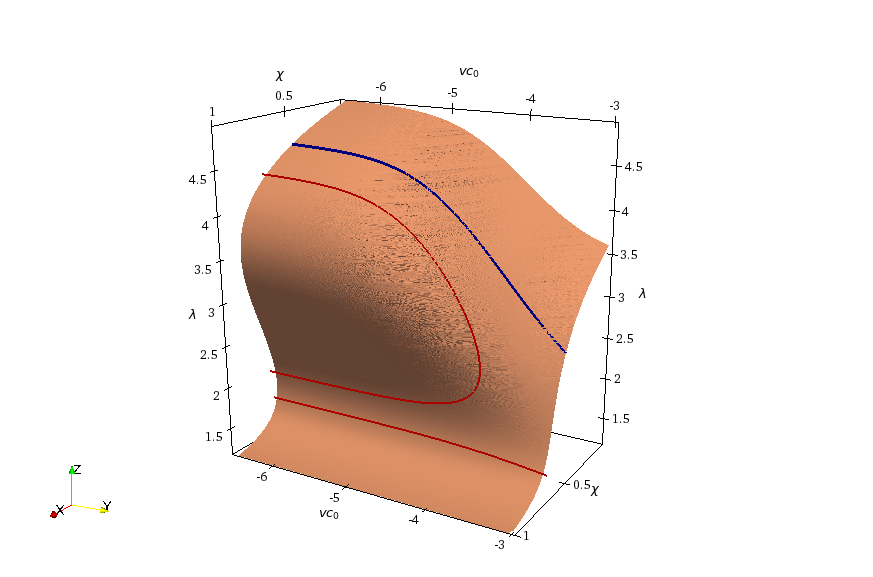
\includegraphics[scale=0.5]{images/manifold1}
	\caption{Two-parameters bifurcation analysis: equilibrium manifold. The red line corresponds to the section of the manifold for $\chi=0.7$, while the blue line $\chi=0.5$.}
	\label{manifold}
\end{figure}
For the free swelling case the deformation tensor $\F=\lambda\mathbb{I}$ so that $\mathbb{B}=\lambda^2\mathbb{I}$. As in the paper by Yu, we now assume that $v=v_s$ so that the equations further simplify to:
\begin{gather}
\begin{aligned}
0 = p v + k_BT\left[2c_0v+\ln \frac{C_s v}{1+C_s v} + \frac{1}{1+C_sv}\right.\label{temp}\\
\left.\ \ \ \ \ \ +\frac{\chi}{(1+C_s v)^2} + \ln \frac{v C_s}{\sum_m v_mC_m}\right], 
\end{aligned}\\[2.5mm]
z_fC_f+C_+-C_-=0,\\
0 = p v \pm e\Phi + 2k_BTc_0+ k_BT \ln \frac{C_\pm}{vc_0\sum_m C_m} ,\\
p= \frac{G}{\lambda^3}\left(\lambda^2-1\right).
\end{gather}
Using Equations(68), we have that the electric potential has the form:
\begin{equation}
\Phi= \frac{k_BT}{2e}\ln\frac{C_-}{C_+}.
\end{equation}
while the concentrations $C_+$ and $C_-$, using also Equation~(\ref{temp}):
\begin{gather}
C_- = c_0 \frac{(v C_s)^2}{1+C_sv} \exp\left(\frac{e\Phi}{k_BT}\right) \exp\left(\frac{1+C_sv+\chi}{(1+vC_s)^2}\right),\\
C_+ = c_0 \frac{(v C_s)^2}{1+C_sv} \exp\left(-\frac{e\Phi}{k_BT}\right) \exp\left(\frac{1+C_sv+\chi}{(1+vC_s)^2}\right),
\end{gather}
which implies that:
\begin{equation}
C_+C_-= c^2_0\frac{(v C_s)^4}{(1+C_sv)^2} \exp\left(2\frac{1+C_sv+\chi}{(1+vC_s)^2}\right).\label{mult}
\end{equation}
Combining~(\ref{mult}) with the electro-neutrality condition, we have:
\begin{equation}
C_\pm = \mp \frac{z_fC_f}{2} + \sqrt{\left( \frac{z_fC_f}{2} \right)^2 + c^2_0\frac{(v C_s)^4}{(1+C_sv)^2} \exp\left(2\frac{1+C_sv+\chi}{(1+vC_s)^2}\right)}.
\end{equation}
Using the incompressibility condition, we have that:
\begin{equation}
\lambda^3=1+vC_s + 2v  \sqrt{\left( \frac{z_fC_f}{2} \right)^2 + c^2_0\frac{(v C_s)^4}{(1+C_sv)^2} \exp\left(2\frac{1+C_sv+\chi}{(1+vC_s)^2}\right)}\label{cond1}.
\end{equation}
Finally substituting the definition of $p$ into Equation~(\ref{temp1}),we have:
\begin{equation}
0=\frac{Gv}{k_BT\lambda^3}(\lambda^2-1) + 2c_0v + \ln \frac{C_sv}{1+C_sv} + \frac{1+vC_s+\chi}{(1+C_sv)^2} + \ln \frac{vC_s}{\lambda^3-1}.\label{cond2}
\end{equation}

Note that the two conditions~(\ref{cond1}) and (\ref{cond2}) uniquely define the equilibrium swelling ration for any value of $c_0$. Fixing the values of the other parameter to match with the work of Yu and varying $vc_0$ and $\chi$, we obtained the manifold showed in Figure \ref{manifold}.

\section{Non-dimensional formulation of the model}
\begin{equation}
D_i=D_i^0,\quad k = \frac{D_0(1+v_sC_s)^\beta}{k_B T c_s} \Rightarrow K=  \frac{D_0(1+v_sC_s)^\beta}{k_B T}.
\end{equation}

Variables rescaling:
\begin{equation*}
\begin{aligned}
k_BT\hat{\mu} + \mu_0 -k_BT= \mu, \qquad \hat{C}_i = vC_i, \qquad \hat{\Phi} = \frac{\Phi e}{k_B T}, \qquad  G_1\hat{p}= p\\
G_1\hat{\mathbb{T}}=\mathbb{T}, \qquad\hat{\mathbf{x}} L =\mathbf{x}, \qquad \hat{t}\tau=t, \qquad e\hat{Q} =v Q, \qquad \hat{K} = \frac{k_BT}{D_0}K
\end{aligned}
\end{equation*}

So that the a-dimensional set of equation is:
\begin{gather}
\begin{aligned}
\mu_s = p \frac{G_1v_s}{k_BT} - \frac{\gamma}{vk_BT L^2} J \nabla^2 C_s + \left[\ln \frac{C_s}{1+C_s} + \frac{1}{1+C_s}\right.\\
\left.\ \ \ \ \ \ +\frac{\chi}{(1+C_s)^2} + \ln \frac{C_s}{\sum_m C_m} \right], 
\end{aligned}\\[2.5mm]
\mu_i = p \frac{G_1v_i}{k_BT} + \Phi z_i + \ln \frac{C_i}{\sum_m C_m} ,\\
-\frac{\epsilon k_B Tv}{L^2e^2} J \nabla^2 \Phi = Q\, \\
\begin{aligned}
\mathbb{T}= -p \mathbb{I} +\frac{\gamma }{G_1v^2L^2} \left[\frac{1}{2} |\nabla C_s|^2\mathbb{I} - \nabla C_s \otimes \nabla C_s\right]+ J^{-1}\left(\mathbb{B}-\mathbb{I}\right)\\
+ \frac{\epsilon k_BT}{L^2e^2} \left[\frac{1}{2} \,|\nabla \Phi|^2\mathbb{I} -\nabla \Phi \otimes \nabla \Phi\right],
\end{aligned}\\
\partial_t C_s=\nabla_0 \cdot\left[\frac{K D_0\tau}{L^2}  \F^{-1}\left(C_s\nabla \mu_s +\sum_i \frac{D_i}{D^0_i} C_i \nabla \mu_i\right)\right],\\
\partial_t C_i= \nabla_0\cdot\left[\frac{D_i\tau}{L^2}C_i\F^{-1}\nabla \mu_i -\frac{D_i}{D^0_i} \frac{C_i}{C_s} \frac{\tau}{L}\mathbf{J}_s\right].
\end{gather}

We consider a 1D problem of constrained swelling, so that the problem simplifies:
\begin{equation}
L_d=\sqrt{\frac{\epsilon k_BTv}{e^2}}<<L \Rightarrow \beta=\frac{L^2_d}{L^2} <<1
\end{equation}
We also assume that:
\begin{equation}
L_{int} = \frac{\gamma}{vk_BT}>L_d
\end{equation}
\begin{gather}
\begin{aligned}
\mu_s = p \mathcal{G} - \frac{L^2_{int}}{L^2}  \partial_Z (J^{-1} \partial_Z C_s) + \left[\ln \frac{C_s}{1+C_s} + \frac{1}{1+C_s}\right.\\
\left.\ \ \ \ \ \ +\frac{\chi}{(1+C_s)^2} + \ln \frac{C_s}{\sum_m C_m} \right], 
\end{aligned}\\[2.5mm]
\mu_i = p \mathcal{G}+ \Phi z_i + \ln \frac{C_i}{\sum_m C_m} ,\\
-\beta^2 \partial_Z (J^{-1}\partial_Z\Phi) = Q\, \\[2.5mm]
T_z= -p - \frac{L^2_i}{2\mathcal{G}L^2} \frac{(\partial_Z C)^2}{J^2}+ J^{-1}\left(J^2-1\right)-\frac{\beta^2}{2v}\frac{(\partial_Z \Phi)^2}{J^2},\\
\partial_t C_s=\partial_Z \cdot\left[\frac{K D_0\tau}{L^2J^2} \left(C_s\partial_Z \mu_s +\sum_i  C_i \partial_Z \mu_i\right)\right],\\
\partial_t C_i= \partial_Z \cdot\left[ \frac{\tau D_0}{L^2J^2} \left(\frac{D_i}{D_0}C_i\partial_Z \mu_i + K C_i \partial_Z\mu_s + K \sum_j \frac{C_jC_i}{C_s}\partial_Z\mu_j\right)\right].
\end{gather}

The time $\tau$ can now be defined as $\tau=L^2/V_0$, where $L$ is the original size of the gel so that $Z=1$ at the boundary. So that:
\begin{gather}
\partial_t C_s=\partial_Z \cdot\left[\frac{K}{J^2} \left(C_s\partial_Z \mu_s +\sum_i  C_i \partial_Z \mu_i\right)\right],\\
\partial_t C_i= \partial_Z \cdot\left[ J^{-2} \left(\frac{D_i}{D_0}C_i\partial_Z \mu_i + K C_i \partial_Z\mu_s + K \sum_j \frac{C_jC_i}{C_s}\partial_Z\mu_j\right)\right].
\end{gather}
We does have that in the external layer, electro neutrality must hold. By expanding the solution in terms of $\beta$ we have at the leading order:
\begin{equation}
Q^0=0 \Longrightarrow \begin{cases}
C_f+\sum_i \left(\sum_m C^0_m\right)c^0_i z_i=0,&\qquad gel\\
\sum_i c^0_i z_i = 0, &\qquad bath
\end{cases}
\end{equation}
which implies the concentration of the ion in the solution $c^0_i$ can not be continuous across the layer. That is why, instead of continuity of the concentration we have continuity of chemical potential.
If we now rescale the space with respect to $\beta$, we have:
\begin{gather}
\begin{aligned}
\mu_s = p \mathcal{G} - \frac{L^2_{int}}{L_d^2}  \partial_Z (J^{-1} \partial_Z C_s) + \left[\ln \frac{C_s}{1+C_s} + \frac{1}{1+C_s}\right.\\
\left.\ \ \ \ \ \ +\frac{\chi}{(1+C_s)^2} + \ln \frac{C_s}{\sum_m C_m} \right], 
\end{aligned}\\[2.5mm]
\mu_i = p \mathcal{G}+ \Phi z_i + \ln \frac{C_i}{\sum_m C_m} ,\\
- \partial_Z (J^{-1}\partial_Z\Phi) = Q\, \\[2.5mm]
T_z= -p - \frac{L^2_i}{2\mathcal{G}L_p^2} \frac{(\partial_Z C)^2}{J^2}+ J^{-1}\left(J^2-1\right)-\frac{1}{2v}\frac{(\partial_Z \Phi)^2}{J^2},\\
\beta\partial_t C_s=\partial_Z \cdot\left[\frac{K D_0\tau}{L^2J^2} \left(C_s\partial_Z \mu_s +\sum_i  C_i \partial_Z \mu_i\right)\right],\\
\beta\partial_t C_i= \partial_Z \cdot\left[ \frac{\tau D_0}{L^2J^2} \left(\frac{D_i}{D_0}C_i\partial_Z \mu_i + K C_i \partial_Z\mu_s + K \sum_j \frac{C_jC_i}{C_s}\partial_Z\mu_j\right)\right].
\end{gather}
So that at first order:
\begin{gather}
0=\partial_Z \cdot\left[\frac{K}{J^2} \left(C_s\partial_Z \mu_s +\sum_i  C_i \partial_Z \mu_i\right)\right],\\
0= \partial_Z \cdot\left[ J^{-2} \left(\frac{D_i}{D_0}C_i\partial_Z \mu_i + K C_i \partial_Z\mu_s + K \sum_j \frac{C_jC_i}{C_s}\partial_Z\mu_j\right)\right].
\end{gather}
Assuming that we are not in the layer where the chemical potential change rapidly because of a change in $C_s$ we have that the derivative of $\mu_m$ needs to tend to zero. So that integrating the above:
\begin{gather}
0=C_s\partial_Z \mu_s +\sum_i  C_i \partial_Z \mu_i \Rightarrow \partial_Z \mu_s=-\sum_i  \frac{C_i}{C_s} \partial_Z \mu_i \\
0=\partial_Z \mu_i \Rightarrow \mu^0_s=const
\end{gather}
So that the chemical potential are constant inside and outside the gel, at first order. Consequently we have that:
\begin{gather}
\begin{aligned}
\mu_s = p \mathcal{G} - \frac{L^2_{int}}{L_d^2}  \partial_Z (J^{-1} \partial_Z C_s) + \left[\ln \frac{C_s}{1+C_s} + \frac{1}{1+C_s}\right.\\
\left.\ \ \ \ \ \ +\frac{\chi}{(1+C_s)^2} + \ln \frac{C_s}{\sum_m C_m} \right], 
\end{aligned}\\[2.5mm]
\mu_i = p \mathcal{G}+ \Phi z_i + \ln \frac{C_i}{\sum_m C_m} ,\\
- \partial_Z (J^{-1}\partial_Z\Phi) = Q\, \\[2.5mm]
\end{gather}
If we also assume that $L_{int}^2/L^2_d>>1$ we must have that at first order:
\begin{equation}
\partial_Z(J^{-1}\partial_ZC^0_s)=0 \Rightarrow \partial_Z C^0_s = J const = \alpha J 
\end{equation}
while the continuity of the stress tensor is given by:
\begin{equation}
-p^{bath}-\frac{\epsilon_r}{2v}\frac{(\partial_Z \Phi)^2}{J^2}=-p - \frac{L^2_i}{2\mathcal{G}L_p^2} \alpha^2 + J^{-1}\left(J^2-1\right)-\frac{1}{2v}\frac{(\partial_Z \Phi)^2}{J^2}
\end{equation}
Also at the first order, have continuity of the electrical potential so that:
\begin{equation}
C^0_i = c^{bath}_0(J-1) \exp\left[\Delta p\mathcal{G}-z_i\Delta \Phi\right]
\end{equation}
where $\Delta=(\cdot)_{bath}-(\cdot)_{gel}$.
In the bath instead the governing equations are:
\begin{gather}
\mu^{b}_s = p^b \mathcal{G} - \frac{L^2_{int,b}}{L^2}  \partial_Z (J^{-1} \partial_Z C_s) + \ln \frac{C_s}{\sum_m C_m}, \\
\mu^{b}_i = p^b \mathcal{G}+ \Phi z_i + \ln \frac{C_i}{\sum_m C_m} ,\\
-\beta^2 \tilde{\epsilon} \partial_Z (J_b^{-1}\partial_Z\Phi) = Q_b\, \\[2.5mm]
T_z= -p - \frac{L^2_{int,b}}{2\mathcal{G}L^2} \frac{(\partial_Z C)^2}{J_{b}^2}-\frac{\beta^2}{2v}\tilde{\epsilon} \frac{(\partial_Z \Phi)^2}{J_b^2},\\
\partial_t C_s=\partial_Z \cdot\left[\frac{K}{J^2} \left(C_s\partial_Z \mu_s +\sum_i  C_i \partial_Z \mu_i\right)\right],\\
\partial_t C_i= \partial_Z \cdot\left[ J_{bath}^{-2} \left(\frac{D_i}{D_0}C_i\partial_Z \mu_i\right].
\end{gather}
%
\subsection{Evolution Equation.}

In order to get a better physical insight into the behaviour, we first rewrite the solvent chemical potential as:
\begin{gather}
\mu_s = \mu^0_s + k_B T \left(\frac{p v_s}{k_BT} +\Pi_{osm}-\sum_i \frac{C_i}{C_s} -\frac{\gamma J}{k_B T}\Pi_{grad}\right)\label{mu2},\\
\Pi_{osm}=\ln \frac{C_s v_s}{1+C_s v_s} + \frac{1}{1+C_sv_s}+\frac{\chi}{(1+C_s v_s)^2},\\
\Pi_{grad} = \nabla^2 C_s,
\end{gather}
where $p$ represents the pore pressure, $\Pi_{osm}$ is the osmotic pressure of the solution and $\Pi_{grad}$ is the pressure due to interface energy. If we now substitute into Equations~(\ref{gov2}) the chemical potentials~(\ref{mu2})-(\ref{mu}), which yields to:
\begin{equation}
\begin{aligned}
\partial_t C_s=\nabla_0 \cdot\left\{K\F^{-1}\left[C_s v_s\nabla p - \color{red}\gamma C_s \nabla J\Pi_{grad}\color{black}+\sum_i \frac{D_i}{D^0_i} C_i e z_i \nabla \Phi\right.\right.\\
\left.\left.+ k_B T\color{teal} \left(C_s \nabla \Pi_{osm}+ \sum_i\left(1-\frac{D_iC_i}{D^0_iC_s}\right) \nabla C_s - \sum_i\left(1-\frac{D_i}{D^0_i}\right) \nabla C_i \right)\color{black}\right]\right\}.\label{long}
\end{aligned}
\end{equation}

The above equation shows that the solvent transport is driven by pressure gradient, osmotic pressure gradient (light-blue term in Equation~(\ref{long})), electric potential gradient and the additional composition gradient (red term in Equation~(\ref{long})), which is here first introduced in the context of polyelectrolytes. In the absence of solutes ($C_i\equiv 0$), we recover the same model presented by Hennessy et. al~\cite{sarah}. 
Similarly we can rewrite Equation~(\ref{gov3}) as:
\begin{equation}
\scriptsize
\partial_t C_i = \nabla_0 \cdot \left[D_i\F^{-1}\left(\underbrace{\nabla C_i}_{\text{diffusion}} +\underbrace{\frac{eC_iz_i}{k_B T} \nabla \Phi}_{\text{electric}}\right)-\underbrace{\frac{D_i C_i}{C_s}\F^{-1}\nabla C_s}_{\text{osmotic pressure}}-\underbrace{\frac{D_i C_i}{D^0_iC_s}\mathbf{J}_s}_{\text{advenction}}\right]\label{long2}
\end{equation}

\subsection{Possible simplification of the model.}

If we consider  the case of small ions, when we can neglect the friction between the ions and the polymer chains, i.e. $D_{i}=D^0_i$. Under this assumption the system of equation simplifies as $K=c_sk$. Following the work of Hennesy et al., we consider the hydraulic permeability $k$ to be:

\begin{equation}
k = \frac{D_0(1+v_sC_s)^\beta}{k_B T c_s} \Rightarrow K=  \frac{D_0(1+v_sC_s)^\beta}{k_B T}.
\end{equation}

The governing equation thus reduces to:
\begin{eqnarray}
\begin{aligned}
\partial_t C_s=\nabla_0 \cdot\left\{\frac{D_0(1+v_sC_s)^\beta}{k_B T}\F^{-1}\left[C_s v_s\nabla p - \gamma C_s \nabla  \left(J\nabla^2 C\right)\right.\right.\\
\left.\left.+\sum_i C_i e z_i \nabla \Phi+ k_B T \left(C_s \nabla \Pi_{osm}+ \sum_i\left(1-\frac{C_i}{C_s}\right) \nabla C_s \right)\right]\right\}.
\end{aligned}\label{A}
\end{eqnarray}
\begin{eqnarray}
\partial_t C_i = \nabla_0 \cdot\left[D_i\F^{-1}\left(\nabla C_i +\frac{eC_iz_i}{k_B T} \nabla \Phi\right)-\frac{D_i C_i}{C_s}\F^{-1}\nabla C_s-\frac{C_i}{C_s}\mathbf{J}_s\right]\label{B}
\end{eqnarray}

\section{1D full model}

Considering a 1D constrained swelling, the deformation gradient tensor is of the form:
\begin{equation}
\F= \begin{bmatrix}
1 & 0 &0\\
0 & 1 &0\\
0 & 0 &J(t,Z)\\
\end{bmatrix}.\label{deffree}                                                                
\end{equation}
where in the dilute case we have $J=1+v_sC_s$.
Similarly all the variables will just depend on the time $t$ and the $Z$ coordinates, the tensor will preserve the same diagonal form, identify by the index $1,2,3$. Given that the set of state and governing equation for the model are given by:

\begin{gather}
\partial_Z S_3 = 0,\\
S_3 = -p - \frac{\gamma}{2} \frac{(\partial_Z C)^2}{J^2} - \frac{\epsilon}{2} \frac{(\partial_Z \Phi)^2}{J^2}+ \frac{G}{J}\left(J^2-1\right),\\[2mm]
-\epsilon \partial_Z \left(J^{-1} \partial_Z \Phi\right)= Q,\\[2mm]
Q= e\left(\sum\limits_{i} z_i C_i + z_fC_f\right)\, ,\\[2mm]
\begin{aligned}
J_s=-\frac{D_0J^{\beta-2}}{k_B T}\left[ - \gamma C_s \partial^2_Z  \left(\frac{\partial_Z C_s}{J}\right)+\sum_i C_i e z_i \partial_Z \Phi+ C_s v_s\partial_Z p\right.\\[2mm]
\left.+ k_B T \left(C_s \partial_Z \Pi_{osm} + \sum_i \left(1-\frac{C_i}{C_s}\right) \partial_Z C_s \right)\right]\, ,
\end{aligned}\\[2mm]
\Pi_{osm}=\ln \frac{C_s v_s}{J} + \frac{1}{J}+\frac{\chi}{J^2},\\[2mm]
\partial_t C_s = -\partial_Z J_s\,,\\[2mm]
\partial_t C_i = \partial_Z \left[\frac{D_i}{J^2}\left(\partial_Z C_i +\frac{eC_iz_i}{k_B T} \partial_Z \Phi\right)-\frac{D_i C_i}{J^2C_s}\partial_Z C_s-\frac{C_i}{C_s}J_s\right]\, .
\end{gather}
 
In the limit of $v_sC_s$
 
\newpage
\bibliographystyle{plain}
\bibliography{ref}
\end{document}